\documentclass[12pt]{report} 
\usepackage{blindtext} 
\usepackage{times} 
\usepackage{graphicx} 
\usepackage{geometry} 
\usepackage{sectsty} 
\usepackage{float} 
\usepackage{array} 
\usepackage[backend=biber,bibencoding=latin1]{biblatex} 
\chapterfont{\centering} 
\usepackage{enumitem} 
\usepackage{enumerate} 
\usepackage{listings} 
\usepackage{color} 
\usepackage{ragged2e} 
\usepackage[headheight=0pt,headsep=0pt]{geometry} 
\definecolor{dkgreen}{rgb}{0,0.6,0} 
\definecolor{gray}{rgb}{0.5,0.5,0.5} 
\definecolor{mauve}{rgb}{0.58,0,0.82} 
\usepackage[table]{xcolor}
\definecolor{lightblue}{HTML}{ADD8E6}
 
  
\lstset{ %   
  language=Java,                  
  basicstyle=\footnotesize,       
  numbers=left,                   
  numberstyle=\tiny\color{gray},  
  stepnumber=1,                   
  numbersep=5pt,                  
  backgroundcolor=\color{white},  
  showspaces=false,               
  showstringspaces=false,         
  showtabs=false,                 
  frame=single,                   
  rulecolor=\color{black},        
  tabsize=2,                      
  captionpos=b,                   
  breaklines=true,                
  breakatwhitespace=false,        
  title=\lstname,                 
  keywordstyle=\color{blue},      
  commentstyle=\color{dkgreen},   
  stringstyle=\color{mauve},      
  escapeinside={\%*}{*)},         
  morekeywords={*,...}            
} 
\geometry{a4paper,total={180mm,250mm},left=20mm,top=20mm, right=20mm} 
\usepackage{indentfirst} 
\thispagestyle{empty} 
\begin{document} 
\newpage
\begingroup
\pagecolor{lightblue} % Set background to black
\color{black}     % Set all text to white
\thispagestyle{empty}

\begin{center}
    \LARGE{\textsc {\textbf{Campus Event Management System: A Monolithic Architecture with Spring Boot and Thymeleaf}}}\\[0.2cm]
    \vspace{0.2cm}
    \Large{\textit{\\School of Computing}}\\[0.3cm]
    
    \Large{\textbf{\\Bachelor of Technology\\in \\Computer Science \& Engineering}}
    \vspace{0.5cm}
    \Large{\textbf{\\By}}\\[0.5cm]
    
    \begin{table}[h] 
    \centering 
    \Large{\color{red} % Ensure table text is white
    \begin{tabular}{>{\bfseries} lc>{\bfseries}r} RAAJI (VTUXXXXX)\\ 
    \end{tabular}} 
    \end{table} 
    
    \large{\textit{10211CSXXX}}\\ 
    \large{\textit{Full Stack Application Development\\ Slot : E1-B2}}\\ 
    \vspace{0.5cm} 
    
    % Logo with white stroke/border
    \fboxsep=5pt % Adjust border padding
   {
\includegraphics[scale=0.5]{Logo.png}}\\ 
    
    \vspace{0.5cm}
    \large{\textbf{DEPARTMENT OF COMPUTER SCIENCE AND ENGINEERING}}\\ 
    \large{\textbf{SCHOOL OF COMPUTING}}\\ 
    \vspace{.5cm}
    \Large{\textbf{VEL TECH RANGARAJAN Dr.SAGUNTHALA R\&D INSTITUTE OF SCIENCE AND TECHNOLOGY\\ (Deemed to be University Estd u/s 3 of UGC Act, 1956)}}\\ 
    \large{\textbf{CHENNAI 600 062, TAMILNADU, INDIA}} 
    \vspace{0.5cm}
    \large{\textbf{\\April, 2026}}\\ 
\end{center} 
\clearpage
\nopagecolor % Revert background to white for the rest of the document
\color{black} % Revert text to black for the rest of the document
\endgroup
 
%CERTIFICATE 
\newpage 
\pagenumbering{roman} 
\begin{center} 
{\Huge \textbf{ BONAFIDE CERTIFICATE}}\\[0.5cm] 
\end{center} 
\linespread{1.5} 
\large{It is certified that the work contained in the Full Stack Application Development \\report titled "Campus Event Management System: A Monolithic Architecture with Spring Boot and Thymeleaf" by Raaji (VTUXXXXX) has been carried out in Winter semester of Academic year 2025-2026(WS2526).} 
\vspace{1.5cm} 
\begin{flushright} 
\textbf{Signature of Faculty\\Dr. Hemamalini.S\\Assistant Professor(Senior Grade)\\Computer Science \& 
Engineering\\School of Computing\\Vel Tech Rangarajan Dr.Sagunthala R\&D\\Institute of Science and Technology\\April, 2026}\\[2.0cm] 
\textbf{Signature of Course Coordinator\\Dr. Sumithra.M\\Assistant Professor(Senior Grade)\\Computer Science \& Engineering\\School of Computing\\Vel Tech Rangarajan Dr.Sagunthala R\&D\\Institute of Science and Technology\\April, 2026}\\  
\end{flushright} 
 
%declaration 
\newpage 
\begin{center} 
\Huge \textbf{DECLARATION} 
\end{center} 
\linespread{1.5} 
\large{ 
 I declare that this written submission represents my ideas in my own words and where others' ideas or words have been included, we have adequately cited and referenced the original sources. I also declare that i have adhered to all principles of academic honesty and integrity and have not misrepresented or fabricated or falsified any idea/data/fact/source in our submission. I understand that any violation of the above will be cause for disciplinary action by the Institute and can also evoke penal action from the sources which have thus not been properly cited or from whom proper permission has not been taken when needed.} 
\vspace{2.0cm} 
\begin{flushright} 
\\ 
\large{(RAAJI)}\\ 
\large{Date:06/05/2026}\\[2.0cm] 
\\ 
\large{}\\ 
\large{}\\[2.0cm] 
\\ 
\large{}\\ 
\large{}\\[2.0cm] 
\end{flushright} 

 

%ABSTRACT 
\newpage 
\begin{center} 
\vspace{2cm} 
\Huge{\textbf{ABSTRACT}}\\[0.5cm] 

\end{center} 
\begin{center} 

\addtocontents{toc}{~\hfill\textbf{Page.No}\par} 

\addcontentsline{toc}{chapter}{ABSTRACT} 
\addtocontents{toc}{\protect\thispagestyle{empty}} 
\end{center} 
\Large{\paragraph  \\The Campus Event Management System is a comprehensive full-stack web application designed to streamline the process of discovering, managing, and registering for events within the campus. Built with a robust Java-based technology stack comprising Spring Boot for the backend and Thymeleaf integrated with Bootstrap 5 for the frontend, the application offers a responsive, user-friendly interface for students and a centralized management dashboard for administrators. Key features include secure administrator authentication using Spring Security, paginated event discovery, automated email confirmations via Spring Boot Starter Mail, and dynamic event creation and tracking. A MySQL database ensures reliable data persistence and maintains relational integrity between administrators, events, and registrations via Spring Data JPA. This project demonstrates the practical implementation of a multi-tier monolithic architecture, DTO pattern mapping, global exception handling, and modern responsive web design principles to deliver a seamless event registration experience.}
 
\vspace{1cm}
\noindent \textbf{Keywords:}  
\textbf{Full-Stack Development, Spring Boot, Thymeleaf, Java, MySQL, Event Management, Spring Security, Monolithic Application.} 
 
 
%list of figure 
\newpage 
 
\renewcommand*\listfigurename{LIST OF FIGURES} 
\addcontentsline{toc}{chapter}{LIST OF FIGURES} 
\listoffigures 

\newpage 
\renewcommand{\listtablename}{LIST OF TABLES} 

\addcontentsline{toc}{chapter}{LIST OF TABLES} 

\listoftables 

 
%list of abbreviation 
\newpage 
\newlist{abbrv}{itemize}{1} 
\setlist[abbrv,1]{label=,labelwidth=1in,align=parleft,itemsep=0.1\baselineskip,leftmargin=!} 
  
\chapter*{LIST OF ACRONYMS AND ABBREVIATIONS} 
\chaptermark{LIST OF ACRONYMS AND ABBREVIATIONS} 
\addcontentsline{toc}{chapter}{LIST OF ACRONYMS AND ABBREVIATIONS} 
\begin{abbrv} 
  
\item[DTO] Data Transfer Object
\item[CRUD] Create, Read, Update, Delete
\item[MVC] Model View Controller
\item[JPA] Java Persistence API
\item[UI] User Interface
\item[ORM] Object Relational Mapping
\item[SQL] Structured Query Language
\item[DI] Dependency Injection

\end{abbrv} 

\newpage 
\renewcommand*\contentsname{TABLE OF CONTENTS} 
%\addtocontents{toc}{\textbf{CONTENT} \hfill \textbf{PAGE NO.}} 
   
\tableofcontents 
 


\addtocontents{toc}{\protect\pagestyle{empty}} 
\thispagestyle{empty} 
 
%introduction 
\chapter{INTRODUCTION} 
\pagenumbering{arabic} 
\section{Introduction}
The rapid digitalization of services has transformed how people interact with events, shifting from manual ticketing systems to centralized online platforms. The Campus Event Management System is developed to address the need for a reliable, scalable, and intuitive system that bridges the gap between event organizers and students. By leveraging modern Java-based web technologies, this platform facilitates seamless event discovery, secure student registration, and hassle-free management processes.
\linespread{1.5} 

\section{Aim of the Project} 
The primary aim of this project is to design and develop a robust web-based application that allows students to easily browse and register for various departmental and institutional events. Additionally, it aims to provide administrators with a powerful, secure dashboard to create, monitor, update, and delete event listings while tracking registration records efficiently.

\section{Scope of the Project} 
The scope of the project encompasses:
\begin{itemize}
    \item A responsive user-facing frontend for browsing events with pagination and search functionalities, and registering for events.
    \item A secure administrative dashboard leveraging Spring Security for comprehensive CRUD operations on events and tracking registrations.
    \item An automated email notification system utilizing Spring Boot Starter Mail to send registration confirmations to students.
    \item A resilient backend utilizing Spring Boot's MVC architecture to handle business logic, DTO mapping, and global exception handling.
    \item A relational database schema utilizing Spring Data JPA (Hibernate) to efficiently store administrator credentials, event details, and registration transactions.
\end{itemize}

\section{Framework} 
The application is built using a modern Java ecosystem tailored for scalable web applications:
\begin{itemize}
    \item \textbf{Frontend:} Thymeleaf templates enhanced with Bootstrap 5 for responsiveness.
    \item \textbf{Backend:} Java 17, Spring Boot 3.x, Spring Web MVC, Spring Security, Spring Boot Mail.
    \item \textbf{Database:} MySQL relational database accessed via Spring Data JPA.
\end{itemize}

\begin{figure}[h]
\centering
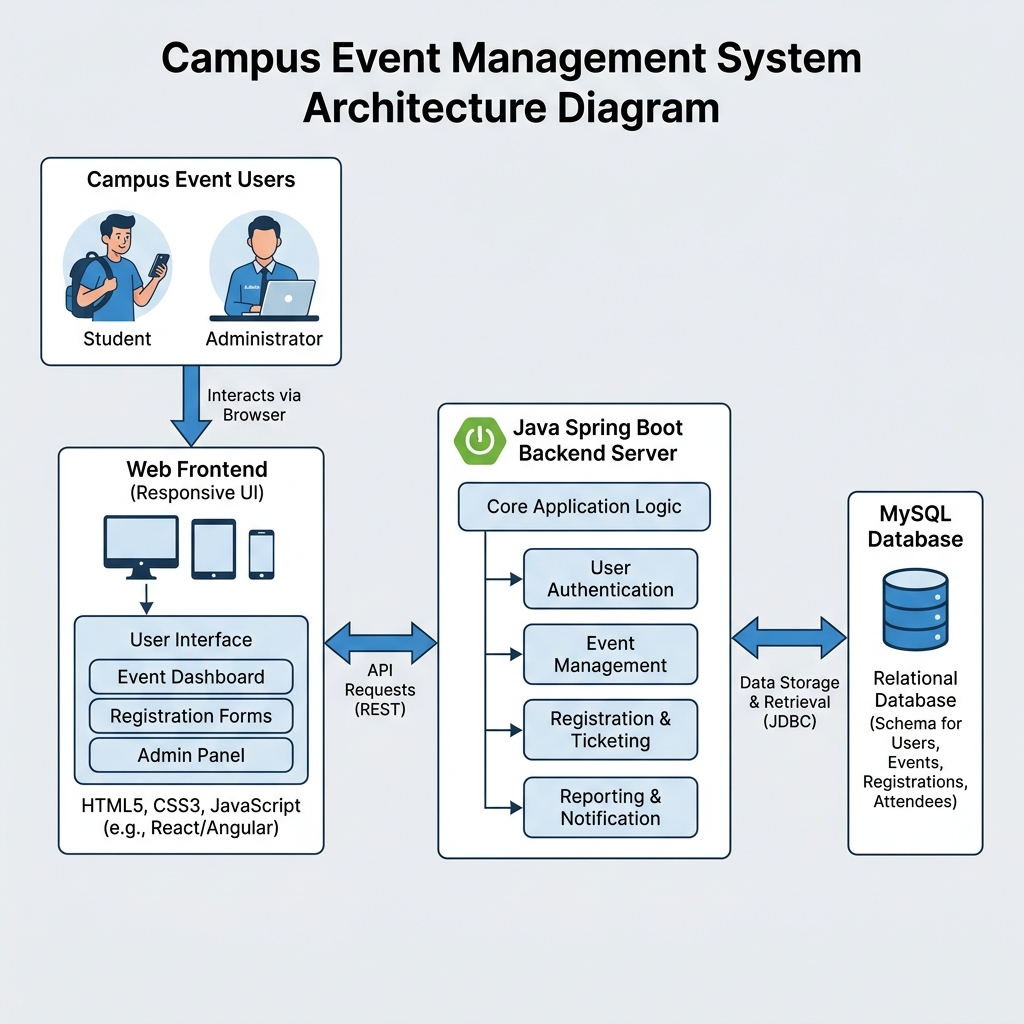
\includegraphics[width=\textwidth,height=0.8\textheight,keepaspectratio]{systemoverview.png}
\caption{System Overview Diagram}
\label{fig:overview}
\end{figure}


\chapter{SURVEY OF SIMILAR APPLICATION IN MARKET} 
The market for event management platforms features industry leaders such as Eventbrite, Meetup, and BookMyShow.
\linespread{1.5} 

\begin{itemize}
    \item \textbf{Eventbrite:} Offers extensive tools for organizers but can be highly complex and introduces significant transaction fees, making it less ideal for localized or institutional campus events.
    \item \textbf{Meetup:} Focuses primarily on community-building and recurring group meetups. It lacks the straightforward registration and tracking structure needed for standalone academic or departmental events.
    \item \textbf{BookMyShow:} A dominant player in the entertainment sector, but its architecture is heavily tailored for large-scale cinema and concert events, making it overkill for campus event management.
\end{itemize}

The proposed Campus Event Management System differentiates itself by offering a lightweight, highly customizable, and cost-effective solution specifically tailored for institutional and departmental events. It eliminates the overhead of enterprise-level platforms while retaining core functionalities.
Additionally, the system provides a simplified, mobile-responsive user interface using Bootstrap 5 and a streamlined workflow ensuring ease of use. Unlike existing platforms that may overwhelm users with unnecessary features, this application focuses strictly on essential functionalities such as event creation, registration, pagination, and search capabilities, making it more accessible for academic organizational use.\vspace{0.5cm}

Furthermore, the application is designed with maintainability in mind, utilizing Java Spring Boot's layered architecture (Controllers, Services, Repositories). This makes the system adaptable to future enhancements, such as payment gateway integrations, while remaining highly performant.


 
%SEMINAR DESCRIPTION 
\chapter{FRAMEWORK DESCRIPTION} 
\linespread{1.5} 
\section{Frontend Implementation} 
\textbf{3.1.1 Environment Setup}

The frontend relies on server-side rendering using Thymeleaf, seamlessly integrated with Spring Boot. Key design dependencies include Bootstrap 5, loaded via CDNs, ensuring modern, responsive UI components without the need for complex Node.js build pipelines.

\textbf{3.1.2 Structure of the Project}

The frontend view templates (located in the \texttt{src/main/resources/templates} directory) are organized intuitively:
\begin{itemize}
    \item \textbf{fragments/}: Contains reusable UI components such as header, navbar, footer, and alert modals.
    \item \textbf{admin/}: Contains protected views for event management, admin user management, and registration tracking.
    \item \textbf{public/}: Contains user-facing views like event catalogs, search results, and registration forms.
\end{itemize}

\textbf{3.1.3 Execution Procedure}

The frontend does not require a separate server execution. It runs embedded within the Spring Boot Tomcat server and is compiled and served automatically when the backend server is launched.


\section{Backend Implementation} 

\textbf{3.2.1 Environment Setup}

The backend is built using the robust Spring Boot framework (Java 17). It relies on Maven for dependency management (\texttt{pom.xml}). Critical dependencies include \texttt{spring-boot-starter-web} for MVC, \texttt{spring-boot-starter-data-jpa} for ORM, \texttt{spring-boot-starter-security} for authentication, and \texttt{spring-boot-starter-mail} for automated emails.

\textbf{3.2.2 Structure of the Project}

The backend architecture rigorously follows a multi-tier structure:
\begin{itemize}
    \item \textbf{model/}: Contains JPA entities mapping to database tables (\texttt{Event}, \texttt{Admin}, \texttt{Registration}).
    \item \textbf{dto/}: Data Transfer Objects ensuring separation between database entities and UI payloads.
    \item \textbf{repository/}: Spring Data JPA interfaces for database CRUD operations.
    \item \textbf{service/}: Contains business logic, email processing, and transactional operations.
    \item \textbf{controller/}: Handles incoming HTTP requests and routes them to appropriate views.
    \item \textbf{config/}: Contains security configurations and component setups.
    \item \textbf{exception/}: Global exception handlers using \texttt{@ControllerAdvice}.
\end{itemize}

\textbf{3.2.3 Execution Procedure}

To execute the application:
1. Ensure a MySQL database server is running locally and the database \texttt{campus\_events} is created.
2. Update the `application.properties` with the correct database credentials.
3. Open the terminal in the project root directory.
4. Execute \texttt{./mvnw spring-boot:run} to start the embedded Tomcat server. The application will be accessible at \texttt{http://localhost:8081}.


\begin{figure}[h]
\centering
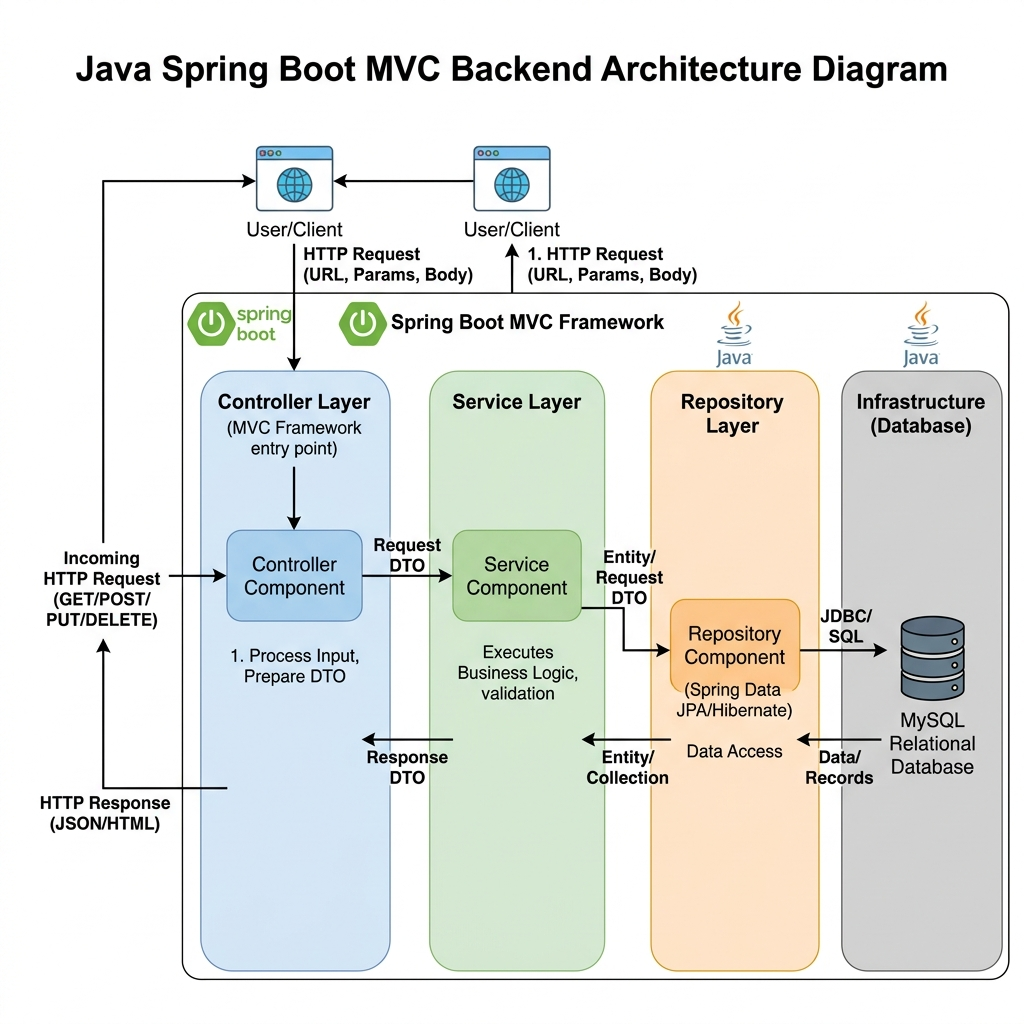
\includegraphics[width=\textwidth,height=0.8\textheight,keepaspectratio]{backend arch.png}
\caption{Backend Architecture}
\label{fig:overview}
\end{figure}


\section{Database Implementation} 
\textbf{3.3.1 Database Configuration}

The application utilizes MySQL for persistent data storage. The connection is managed via HikariCP and Spring Data JPA via JDBC. The connection parameters are specified in the \texttt{application.properties} file.

\textbf{3.3.2 Schema Structure}

The schema is relationally designed and automatically generated and updated via Hibernate (\texttt{spring.jpa.hibernate.ddl-auto=update}).

\textbf{3.3.3 Tables Created}

\begin{itemize}
    \item \textbf{admin}: Stores administrator credentials securely. Columns include ID, Username, and Password (managed via Spring Security).
    \item \textbf{event}: Stores event details. Columns include ID, Name, Description, Date, Time, Venue, and Total Capacity.
    \item \textbf{registration}: Stores student registration records. Columns include ID, Student Name, Student Email, Registration Date, and a foreign key linking to the \texttt{event} table.
\end{itemize}

\chapter{ METHODOLOGIES } 
\linespread{1.5} 
\section{Project Architecture} 
  
The project follows a Monolithic Model-View-Controller (MVC) architecture. Incoming client requests are handled by the Spring DispatcherServlet, which routes them to the appropriate Controller. Controllers interact with Service layers via Dependency Injection, which in turn use Repositories for data access. Processed data is then bound to Thymeleaf views and returned as formatted HTML to the client browser.

\section{DataFlow Diagram} 
1. The User interacts with the UI to submit a registration form. \\
2. The browser sends an HTTP POST request to the corresponding Controller mapping. \\
3. The Controller validates the input data against the DTO. If valid, it invokes the Service layer. \\
4. The Service layer executes business logic and interacts with the JPA Repository to save the \texttt{Registration} entity. \\
5. An automated confirmation email is queued and dispatched asynchronously via Spring Boot Mail. \\
6. The user is redirected to a success view with a confirmation message.

\section{Module 1: Administrator Authentication} 
This module is a critical security component that leverages the robust capabilities of Spring Security to rigorously restrict access to sensitive administrative endpoints and management URLs. It establishes a secure gateway utilizing form-based authentication, which intercepts unauthorized requests and seamlessly redirects them to a dedicated login portal. Behind the scenes, the module actively manages user sessions, tracking authenticated states to prevent session hijacking and cross-site request forgery (CSRF) vulnerabilities. User credentials are securely managed and authenticated against backend records, adhering to industry best practices for data protection. Furthermore, the authentication mechanism ensures that only authorized personnel with verified administrative privileges can access the core functionalities of the system. This includes safeguarding the event creation dashboard, modifying existing event records, and accessing comprehensive registration tracking tools. By implementing stringent access control, the system maintains strict data integrity and operational security, guaranteeing that the management infrastructure remains impenetrable to unauthorized users and automated malicious bots.

\section{Module 2: Event Management \& Discovery} 
Serving as the operational core of the application, this module provides administrators with a comprehensive suite of tools to execute full CRUD (Create, Read, Update, Delete) operations on event records. Through an intuitive, Bootstrap-powered dashboard, organizers can seamlessly generate new event listings by specifying critical details such as event titles, detailed descriptions, precise scheduling, venue locations, and maximum attendee capacities. Conversely, on the public-facing side, the module delivers an optimized event discovery experience for students. To handle extensive datasets efficiently, it incorporates advanced server-side pagination utilizing Spring Data JPA, ensuring that the user interface remains responsive and lightweight, even when rendering hundreds of active events. Additionally, a robust search mechanism empowers users to filter events dynamically based on relevant keywords or categories. This dual-faceted approach guarantees that administrators possess the necessary granular control to manage institutional schedules, while simultaneously providing students with a fast, intuitive, and accessible catalog to explore upcoming campus activities without experiencing performance bottlenecks.

\section{Module 3: Registration \& Notification System} 
This module facilitates the entire student enrollment workflow, serving as the bridge between user intent and successful event participation. When a student initiates a registration request, the system actively performs real-time capacity validation against the backend MySQL database, ensuring that the selected event has not exceeded its predefined maximum attendance limit. Upon successful validation, the module securely records the participant's details, persisting the transactional data via Hibernate ORM to maintain relational integrity between the student and the event. Immediately following a successful database commit, the system leverages Spring Boot Starter Mail to asynchronously dispatch a personalized booking confirmation email to the user via an integrated SMTP service, providing immediate digital verification of their reserved slot. To enhance system resilience, the module incorporates comprehensive global exception handling utilizing the @ControllerAdvice annotation. This sophisticated error-management architecture guarantees that any registration anomalies---such as attempting to book a fully-booked event or submitting invalid email formats---are gracefully intercepted. Consequently, users are presented with clear, actionable, and user-friendly alert notifications instead of technical stack traces.

\vspace{0.5cm}
\textbf{Advantages of this Project} 

\begin{itemize}
    \item \textbf{Robustness:} The statically typed nature of Java and the comprehensive ecosystem of Spring Boot provide a highly reliable foundation.
    \item \textbf{SEO Friendly:} Server-side rendering with Thymeleaf provides fully populated HTML directly to the browser, significantly enhancing search engine optimization.
    \item \textbf{Maintainability:} The rigid enforcement of the MVC pattern and DTOs prevents spaghetti code and facilitates future upgrades.
\end{itemize}


\vspace{0.5cm}
\textbf{Disadvantages} 

\begin{itemize}
    \item \textbf{Monolithic Coupling:} Unlike decoupled frontend/backend applications, the UI and API logic are tightly coupled in the same deployment unit, making it slightly harder to scale independently.
    \item \textbf{Server Load:} Server-side rendering consumes more server CPU and memory compared to delivering a static Single Page Application (SPA).
\end{itemize}
\vspace{0.3cm}

This project emphasizes clean coding practices such as Dependency Injection and aspect-oriented exception handling. The Bootstrap 5 integration ensures the application remains highly accessible across diverse devices. 

\chapter{RESULTS AND DISCUSSIONS} 
\linespread{1.5} 
The Campus Event Management System successfully fulfills its functional requirements. Students can intuitively navigate the platform, utilize the search and pagination tools to discover events, and register seamlessly. Administrators possess reliable oversight over event listings via a secured dashboard. 

The integration of Thymeleaf provides fast, responsive page loads. The Spring Boot backend efficiently processes form submissions, and the MySQL database accurately maintains data integrity. Email confirmations dispatch reliably. \\

\begin{table}[H]
\centering
\small
\renewcommand{\arraystretch}{1.3}
\begin{tabular}{|p{3.5cm}|p{3cm}|p{3cm}|p{3cm}|}
\hline
\textbf{Feature} & \textbf{Eventbrite} & \textbf{BookMyShow} & \textbf{Proposed App} \\
\hline
Custom Branding & Limited & Limited & High \\
\hline
Transaction Fees & High & Moderate & None (Self-Hosted) \\
\hline
Setup Complexity & High & Moderate & Low \\
\hline
Target Audience & Commercial Events & Entertainment Sector & Institutional / Departmental \\
\hline
Data Ownership & Third-Party & Third-Party & Fully Owned \\
\hline
Architecture & Microservices & Microservices & Monolithic MVC \\
\hline
Cost Efficiency & Low & Moderate & High \\
\hline
\end{tabular}
\caption{Application Feature Comparison}
\end{table}

\vspace{0.5cm}
\noindent As illustrated in the Application Feature Comparison table above, the proposed Campus Event Management System provides significant advantages for institutional use over existing commercial platforms. While applications like Eventbrite and BookMyShow excel in the commercial and entertainment sectors, they often impose high transaction fees, limited branding capabilities, and complex setups. In contrast, our proposed system is tailored specifically for academic and departmental needs. By utilizing a self-hosted monolithic MVC architecture, it completely eliminates transaction fees, guarantees full data ownership, and drastically reduces setup complexity. This ensures a highly cost-effective and customizable solution that directly aligns with the operational requirements of campus event management.
\vspace{0.5cm}

\section{System Screenshots and Results}

The developed application is currently deployed in a local environment (localhost:8081) and includes the following views:

% -------- PAGE 1 --------

\subsection{Admin Login Page}

This secure portal limits access to the event management systems, governed by Spring Security.

\begin{figure}[H]
\centering
\includegraphics[width=0.7\textwidth]{FSAD SC/login.png}
\caption{Admin Login Page}
\end{figure}

\vspace{0.3cm}
\noindent \textbf{Description:} The figure above illustrates the secure login portal designed exclusively for administrators. Built with Bootstrap 5, the interface provides a clean, responsive layout where authorized personnel must authenticate themselves using valid credentials. This gateway is rigorously protected by Spring Security, which intercepts all unauthorized attempts to access the management dashboard, ensuring that only authenticated users can manipulate campus event data.

\subsection{Event Discovery Portal}

Displays available events to students with server-side pagination and search capabilities.

\begin{figure}[H]
\centering
\includegraphics[width=0.7\textwidth]{FSAD SC/register.png}
\caption{Event Discovery Portal}
\end{figure}

\vspace{0.3cm}
\noindent \textbf{Description:} The figure above displays the primary user-facing interface where students can browse upcoming campus events. The portal features a dynamic search bar for filtering events by name or category, and implements server-side pagination to handle large volumes of data without browser lag. Each event card provides essential details such as date, venue, and a direct link to the registration page, offering an intuitive and engaging user experience.

\newpage

% -------- PAGE 2 --------

\subsection{Admin Dashboard}

Provides an overview for administrators to add, edit, and delete events, as well as track registration counts.

\begin{figure}[H]
\centering
\includegraphics[width=\textwidth]{FSAD SC/admin dashboard.png}
\caption{Admin Dashboard}
\end{figure}

\vspace{0.3cm}
\noindent \textbf{Description:} The figure above showcases the comprehensive Admin Dashboard, serving as the central control panel for event management. From this interface, administrators can easily perform full CRUD operations---creating new events, modifying existing details, or deleting outdated listings. The dashboard also provides real-time tracking of registration metrics, allowing organizers to monitor attendance limits and manage student enrollment efficiently from a unified, easily accessible view.
\newpage
\subsection{Event Registration Page}

Allows students to input their details to register for a specific event. Includes DTO-based form validation.
\\
\begin{figure}[H]
\centering
\includegraphics[width=\textwidth]{FSAD SC/booking page.png}
\caption{Event Registration Interface}
\end{figure}

\vspace{0.3cm}
\noindent \textbf{Description:} The figure above depicts the dedicated event registration form utilized by students to secure their participation. The form incorporates rigorous DTO-based validation to ensure all submitted data, such as the student's email and identification number, is accurately formatted. Upon submission, the system actively performs a real-time capacity check against the backend database before confirming the booking and triggering an automated SMTP confirmation email to the participant.

\newpage


\chapter{CONCLUSION AND FUTURE ENHANCEMENTS}

\section{Conclusion}

The Campus Event Management System demonstrates the continued effectiveness of server-side rendered architectures using modern Java frameworks. By integrating Spring Boot, Thymeleaf, Spring Security, and MySQL, the system provides a robust, fast, and accessible platform for managing institutional events.

The application successfully implements complex backend functionalities like DTO mappings, transactional safety, and global error handling, while offering an attractive frontend powered by Bootstrap 5.

\section{Future Enhancements}

\begin{itemize}

\item \textbf{RESTful API Transition:} Decouple the application by exposing REST endpoints and migrating the frontend to a SPA framework like React or Angular.

\item \textbf{QR Code Check-ins:} Generate dynamic QR codes and email them to students for fast physical check-in at event venues.

\item \textbf{Advanced Analytics:} Implement charting libraries in the admin dashboard to visualize event popularity and attendance trends.

\item \textbf{Dockerization:} Containerize the application using Docker to streamline deployment processes to cloud environments.

\end{itemize}

\section{Existing Applications and Review}

\begin{itemize}

\item \textbf{Eventbrite} \\
\url{https://www.eventbrite.com} \\
Eventbrite is a widely used event management platform that provides ticketing, analytics, and promotion tools. However, it involves service charges and may be complex for beginners.

\item \textbf{BookMyShow} \\
\url{https://in.bookmyshow.com} \\
BookMyShow is popular in India for booking movie and event tickets. It offers a smooth user interface but is mainly focused on entertainment events.

\item \textbf{Meetup} \\
\url{https://www.meetup.com} \\
Meetup enables users to join communities and attend events. It is useful for networking but lacks strong ticketing and payment integration.

\end{itemize}

\newpage
\chapter{ADDRESSING COMPLEX ENGINEERING PROBLEM AND SDG}

\section{Mapping of the Project to Complex Engineering Problem (CEP)}

\begin{table}[h!]
\centering
\footnotesize
\renewcommand{\arraystretch}{1.3}
\begin{tabular}{|p{1.2cm}|p{2.8cm}|p{4cm}|p{1.5cm}|p{5cm}|}
\hline
\textbf{Level} & \textbf{Attribute} & \textbf{Characteristics} & \textbf{WKs} & \textbf{Justification} \\
\hline
WP1 & Depth of Knowledge & Requires in-depth engineering & WK4, WK5 & Knowledge of Spring Boot, MVC, DTOs, Security \\
\hline
WP2 & Conflicting Requirements & Technical and non-technical constraints & WK4, WK5 & Balances system performance with full page reloads \\
\hline
WP3 & Depth of Analysis & Analytical and design thinking & WK3, WK4 & Relational schema design, entity mapping \\
\hline
WP4 & Familiarity & Partially new problems & WK4 & Exception handling across layers \\
\hline
WP5 & Applicable Codes & Limited standard solutions & WK6 & Custom security filter chains \\
\hline
WP6 & Stakeholder Needs & Multiple stakeholders & WK5, WK6 & Students, faculty, organizers \\
\hline
WP7 & Interdependence & System-level integration & WK3, WK5 & UI + Service + Database integration \\
\hline
\end{tabular}
\caption{Mapping of CEP Attributes}
\end{table}

\vspace{0.5cm}

\section{Mapping of the Project to Complex Engineering Activities (CEA)}

\begin{table}[h!]
\centering
\footnotesize
\renewcommand{\arraystretch}{1.3}
\begin{tabular}{|p{1.5cm}|p{3cm}|p{4.5cm}|p{5cm}|}
\hline
\textbf{EA No.} & \textbf{Attribute} & \textbf{Characteristics} & \textbf{Justification} \\
\hline
EA1 & Range of Resources & Use of technologies & Java, Spring Boot, MySQL, Bootstrap \\
\hline
EA2 & Level of Interactions & Complex module interaction & Controller + Service + Repository \\
\hline
EA3 & Innovation & Modern technologies & Spring Data JPA, automated emailing \\
\hline
EA4 & Consequences & Impact on users & Simplifies registration \\
\hline
EA5 & Familiarity & Beyond standard & Robust server-side rendering \\
\hline
\end{tabular}
\caption{Mapping of CEA Attributes}
\end{table}

\vspace{0.5cm}

\section{SDG Mapping (CEP Section)}

\begin{table}[h!]
\centering
\footnotesize
\renewcommand{\arraystretch}{1.3}
\begin{tabular}{|p{2cm}|p{4cm}|p{7cm}|}
\hline
\textbf{SDG No.} & \textbf{SDG Title} & \textbf{Relevance} \\
\hline
SDG 4 & Quality Education & Supports academic events and learning platforms \\
\hline
SDG 9 & Innovation & Promotes use of modern Java frameworks \\
\hline
SDG 10 & Reduced Inequalities & Accessible, highly responsive system for all users \\
\hline
SDG 11 & Sustainable Communities & Encourages organized and efficient campus event management \\
\hline
\end{tabular}
\caption{SDG Mapping}
\end{table}
\newpage
\chapter*{REFERENCES}
\addcontentsline{toc}{chapter}{References}

\begin{enumerate}

\item Spring Boot Documentation: \url{https://spring.io/projects/spring-boot}

\item Thymeleaf Documentation: \url{https://www.thymeleaf.org/documentation.html}

\item Spring Security Reference: \url{https://docs.spring.io/spring-security/reference/index.html}

\item Spring Data JPA: \url{https://spring.io/projects/spring-data-jpa}

\item Bootstrap 5 Documentation: \url{https://getbootstrap.com/docs/5.0/getting-started/introduction/}

\item Hibernate ORM: \url{https://hibernate.org/orm/documentation/}

\item Java Platform, Standard Edition Documentation: \url{https://docs.oracle.com/en/java/javase/17/}

\end{enumerate}
\end{document}